\documentclass[a4paper,oneside,11pt]{book}

% =========================================================
% PACKAGE
% =========================================================

\usepackage{graphicx}
\usepackage{titling}
\usepackage[indonesian]{babel}
\usepackage{titlesec}
\usepackage{geometry}
\usepackage{setspace}
\usepackage{fancyhdr}
\usepackage{hyperref}
\usepackage{listings}
\usepackage{xcolor}
\usepackage{float}
\usepackage{tocloft}
\usepackage{lipsum}
\usepackage{indentfirst}

% =========================================================
% PAGE SETUP
% =========================================================

\geometry{
    left=3cm,
    right=2cm,
    top=2cm,
    bottom=2cm
}

\onehalfspacing
\setlength{\headheight}{14pt}

% =========================================================
% CHAPTER FORMAT
% =========================================================

\titleformat{\chapter}
    {\normalfont\bfseries\centering}
    {Bab \thechapter.}
    {0.5em}
    {}

\titlespacing*{\chapter}
    {0pt}
    {0pt}
    {20pt}

% =========================================================
% SECTION FORMAT
% =========================================================

\titleformat{\section}
    {\normalfont\bfseries}
    {\thesection}
    {0.5em}
    {}

\titleformat{\subsection}
    {\normalfont\bfseries}
    {\thesubsection}
    {0.5em}
    {}

% =========================================================
% HEADER & FOOTER
% =========================================================

\pagestyle{fancy}
\fancyhf{}
\fancyhead[L]{Laporan Praktikum}
\fancyhead[R]{Pemrograman Perangkat Bergerak Dasar}
\fancyfoot[C]{\thepage}

\renewcommand{\headrulewidth}{0.4pt}
\renewcommand{\footrulewidth}{0pt}

% =========================================================
% WARNA KODE
% =========================================================

\definecolor{codeRed}{RGB}{190,40,50}
\definecolor{codeBlue}{RGB}{45,80,160}
\definecolor{codeGreen}{RGB}{45,120,70}
\definecolor{codeGray}{RGB}{100,100,100}

% =========================================================
% KOTLIN
% =========================================================

\lstdefinelanguage{Kotlin}{
    morekeywords={
        package,
        import,
        class,
        object,
        fun,
        val,
        var,
        private,
        public,
        protected,
        internal,
        override,
        lateinit,
        this,
        return,
        if,
        else,
        when,
        for,
        while,
        in,
        is,
        null,
        true,
        false
    },
    sensitive=true,
    morecomment=[l]{//},
    morecomment=[s]{/*}{*/},
    morestring=[b]"
}

% =========================================================
% XML
% =========================================================

\lstdefinelanguage{MyXML}{
    morecomment=[s]{<!--}{-->},
    morestring=[b]"
}

% =========================================================
% FORMAT KODE
% =========================================================

\lstset{
    basicstyle=\ttfamily\scriptsize,
    numbers=left,
    numberstyle=\tiny\color{codeGray},
    numbersep=7pt,
    frame=single,
    rulecolor=\color{black},
    breaklines=true,
    breakatwhitespace=false,
    columns=fullflexible,
    keepspaces=true,
    showstringspaces=false,
    tabsize=4,
    xleftmargin=18pt,
    framexleftmargin=12pt,
    aboveskip=8pt,
    belowskip=8pt
}

% =========================================================
% KHUSUS KOTLIN
% =========================================================

\lstdefinestyle{kotlinstyle}{
    language=Kotlin,
    keywordstyle=\color{codeBlue},
    stringstyle=\color{codeRed},
    commentstyle=\color{codeGreen},
    identifierstyle=\color{black}
}

% =========================================================
% KHUSUS XML
% =========================================================

\lstdefinestyle{xmlstyle}{
    language=MyXML,
    keywordstyle=\color{black},
    stringstyle=\color{codeRed},
    commentstyle=\color{codeGreen},
    identifierstyle=\color{black}
}

% =========================================================
% TABLE OF CONTENTS
% =========================================================

\renewcommand{\contentsname}{Daftar Isi}

% =========================================================
% DOCUMENT
% =========================================================


\begin{document}
\hypersetup{hypertexnames=false,hidelinks}
\setlength{\emergencystretch}{3em}
\renewcommand{\cftchappresnum}{Bab }
\renewcommand{\cftchapaftersnum}{. }
\setlength{\cftchapnumwidth}{3.8em}
\hypersetup{pageanchor=false}
\begin{titlepage}
\begin{center}
\vspace*{0.9cm}
{\fontsize{14.4}{17.5}\selectfont\bfseries
Laporan Praktikum\par
Pemrograman Perangkat Bergerak Dasar\par
Pertemuan 5\par
Spinner, Date Picker, Time Picker, Dialog\par}
\vspace{1cm}

\includegraphics[width=8cm]{lambang ugm.png}\par
\vspace{1cm}
{\fontsize{12}{17}\selectfont
Nama Mahasiswa: Reyhan Abelard Fikri\par
NIM: 25/562000/SV/26713\par
Kelas: A1\par
\vspace{0.5cm}
Dosen Pengampu:\par
Dr. Irkham Huda, S.Kom., M.Cs.\par}
\vfill
{\fontsize{14.4}{17.5}\selectfont\bfseries
Sekolah Vokasi\par
Universitas Gadjah Mada\par
Yogyakarta\par
2026\par}
\end{center}
\end{titlepage}
\hypersetup{pageanchor=true}
\tableofcontents
\clearpage

\chapter{Tujuan Praktikum}
\begin{enumerate}
\item Memahami penggunaan \textit{Spinner} untuk memilih status presensi pada aplikasi Android.
\item Menerapkan \textit{DatePicker} dan \textit{TimePicker} untuk membaca tanggal serta waktu yang dipilih pengguna.
\item Menghubungkan layout XML dengan kode Kotlin menggunakan \textit{View Binding}, mengatur kolom keterangan berdasarkan status, dan memvalidasi input presensi.
\item Membuat \textit{custom dialog} sebagai konfirmasi keluar dari aplikasi serta memeriksa fungsi tombol Ya dan Tidak.
\end{enumerate}

\chapter{Hasil dan Pembahasan}
\section{Langkah-Langkah Praktikum}
\subsection{Membuat Project dan Mengaktifkan View Binding}
Project baru dibuat melalui \textit{New Project} pada Android Studio dengan template \textit{Empty Views Activity}. Project diberi nama \texttt{PresensiApp}, menggunakan bahasa Kotlin, package \texttt{com.example.presensiapp}, dan minimum SDK API 24. Template ini menyediakan Activity Kotlin dan layout XML yang diperlukan untuk latihan pada modul.

Pada file \texttt{app/build.gradle.kts}, \textit{View Binding} diaktifkan di dalam blok \texttt{android}. Setelah konfigurasi ditambahkan, project disinkronkan melalui \textit{Sync Now}. Konfigurasi yang digunakan adalah sebagai berikut.
\begin{lstlisting}[style=kotlinstyle]
buildFeatures {
    viewBinding = true
}
\end{lstlisting}
Build menggunakan SDK yang terpasang pada komputer, yaitu compile SDK dan target SDK 37, sementara minimum SDK tetap API 24 sesuai modul. Pengujian tampilan dilakukan pada emulator Pixel 8 Pro. Perintah \texttt{assembleDebug} selesai dengan status \texttt{BUILD SUCCESSFUL} dan menghasilkan APK debug yang dapat dipasang pada emulator.

\subsection{Menyusun Tampilan Presensi}
Tampilan utama disusun pada \texttt{activity\_main.xml}. \textit{ScrollView} memungkinkan pengguna menggulir halaman ketika kolom keterangan atau hasil presensi menambah tinggi tampilan. Di dalamnya terdapat \textit{LinearLayout} vertikal yang memuat judul Presensi, \textit{DatePicker} mode kalender, \textit{TimePicker} mode spinner, pilihan status, kolom keterangan, tombol Submit, tombol Keluar, dan teks hasil.

Kolom keterangan memiliki nilai awal \texttt{gone}. Dengan demikian, status awal Hadir Tepat Waktu tidak menampilkan kolom tersebut. Teks hasil juga disembunyikan sampai input berhasil dikirim. Kode layout yang digunakan adalah sebagai berikut.
\lstinputlisting[style=xmlstyle]{kode/activity_main.xml}

\subsection{Menyiapkan Pilihan Status}
Empat pilihan status didefinisikan melalui \texttt{string-array} di \texttt{strings.xml}, yaitu Hadir Tepat Waktu, Sakit, Terlambat, dan Izin. File ini juga menyimpan label tampilan serta pesan validasi dan konfirmasi.
\lstinputlisting[style=xmlstyle]{kode/strings.xml}

Pada \texttt{MainActivity}, daftar dibaca dengan \texttt{getStringArray()} dan dimasukkan ke \texttt{ArrayAdapter}. Layout \texttt{simple\_spinner\_item} digunakan untuk pilihan aktif, sedangkan \texttt{simple\_spinner\_dropdown\_item} digunakan untuk daftar pilihan saat Spinner dibuka.

\subsection{Menghubungkan Layout dan Mengatur Input Presensi}
\texttt{ActivityMainBinding.inflate(layoutInflater)} membentuk binding dari layout, kemudian \texttt{setContentView(binding.root)} menampilkan halaman. Akses ke komponen dilakukan melalui binding, misalnya \texttt{binding.datePicker} dan \texttt{binding.spinnerStatus}. Penanganan \textit{window insets} memberikan ruang untuk status bar dan navigation bar agar konten tidak tertutup.

\texttt{OnItemSelectedListener} memeriksa posisi status. Posisi nol merupakan Hadir Tepat Waktu, sehingga label serta input keterangan disembunyikan dan input lama dikosongkan. Pada posisi lainnya, keduanya ditampilkan. Aturan ini diterapkan pada Sakit, Terlambat, dan Izin.

Saat Submit ditekan, aplikasi membaca status serta keterangan yang telah dirapikan dengan \texttt{trim()}. Jika status selain Hadir Tepat Waktu belum memiliki keterangan, \texttt{EditText.error} menampilkan pesan ``Isi keterangan terlebih dahulu'' dan proses dihentikan dengan \texttt{return}.

Jika input valid, tanggal dibaca dari \texttt{dayOfMonth}, \texttt{month}, dan \texttt{year}. Nilai bulan ditambah satu karena \texttt{DatePicker.month} memakai indeks nol. Waktu dibaca melalui \texttt{hour} dan \texttt{minute}, kemudian diubah ke format dua belas jam dengan AM atau PM. Aplikasi menampilkan notifikasi \textit{Toast} dan ringkasan pada \textit{TextView} supaya hasil tetap dapat dibaca setelah Toast menghilang. Keterangan hanya ditambahkan untuk status yang memerlukannya.

Tombol Keluar dan tombol Back menampilkan dialog konfirmasi. Pemeriksaan tag dialog mencegah dialog yang sama dibuka berulang. Ringkasan hasil juga dimasukkan ke \texttt{savedInstanceState} untuk mempertahankannya saat Activity dibuat ulang. Kode \texttt{MainActivity.kt} yang digunakan adalah sebagai berikut.
\lstinputlisting[style=kotlinstyle]{kode/MainActivity.kt}

\subsection{Membuat Custom Dialog Keluar}
Layout \texttt{dialog\_exit.xml} memuat judul ``Keluar aplikasi?'', pesan konfirmasi, serta tombol Tidak dan Ya. Layout dihubungkan menggunakan \texttt{DialogExitBinding}, sehingga bentuk dialog berasal dari layout yang dibuat sendiri.
\lstinputlisting[style=xmlstyle]{kode/dialog_exit.xml}

Class \texttt{DialogExit} mewarisi \texttt{DialogFragment}. \texttt{AlertDialog.Builder} menerima layout melalui \texttt{setView()}. Tombol Tidak menjalankan \texttt{dismiss()} untuk menutup dialog, sedangkan tombol Ya memanggil \texttt{finish()} untuk menutup Activity.
\lstinputlisting[style=kotlinstyle]{kode/DialogExit.kt}

\section{Hasil Pengujian Aplikasi}
Pengujian dilakukan dengan menjalankan APK pada emulator. Bukti berikut merupakan screenshot dari aplikasi yang telah dibuat. Tanggal dipilih menjadi 28 September 2026 dan waktu diubah menjadi 06:34 AM untuk memastikan nilai pilihan dibaca pada hasil Submit. Pengujian ini memakai data contoh untuk demonstrasi.

\subsection{Tampilan Awal dan Daftar Status}
Pada tampilan awal, DatePicker, TimePicker, Spinner, tombol Submit, dan tombol Keluar dapat digunakan. Status awal Hadir Tepat Waktu tidak menampilkan kolom keterangan. Saat Spinner dibuka, empat pilihan status muncul.
\begin{figure}[H]
\centering
\begin{minipage}{0.46\textwidth}\centering
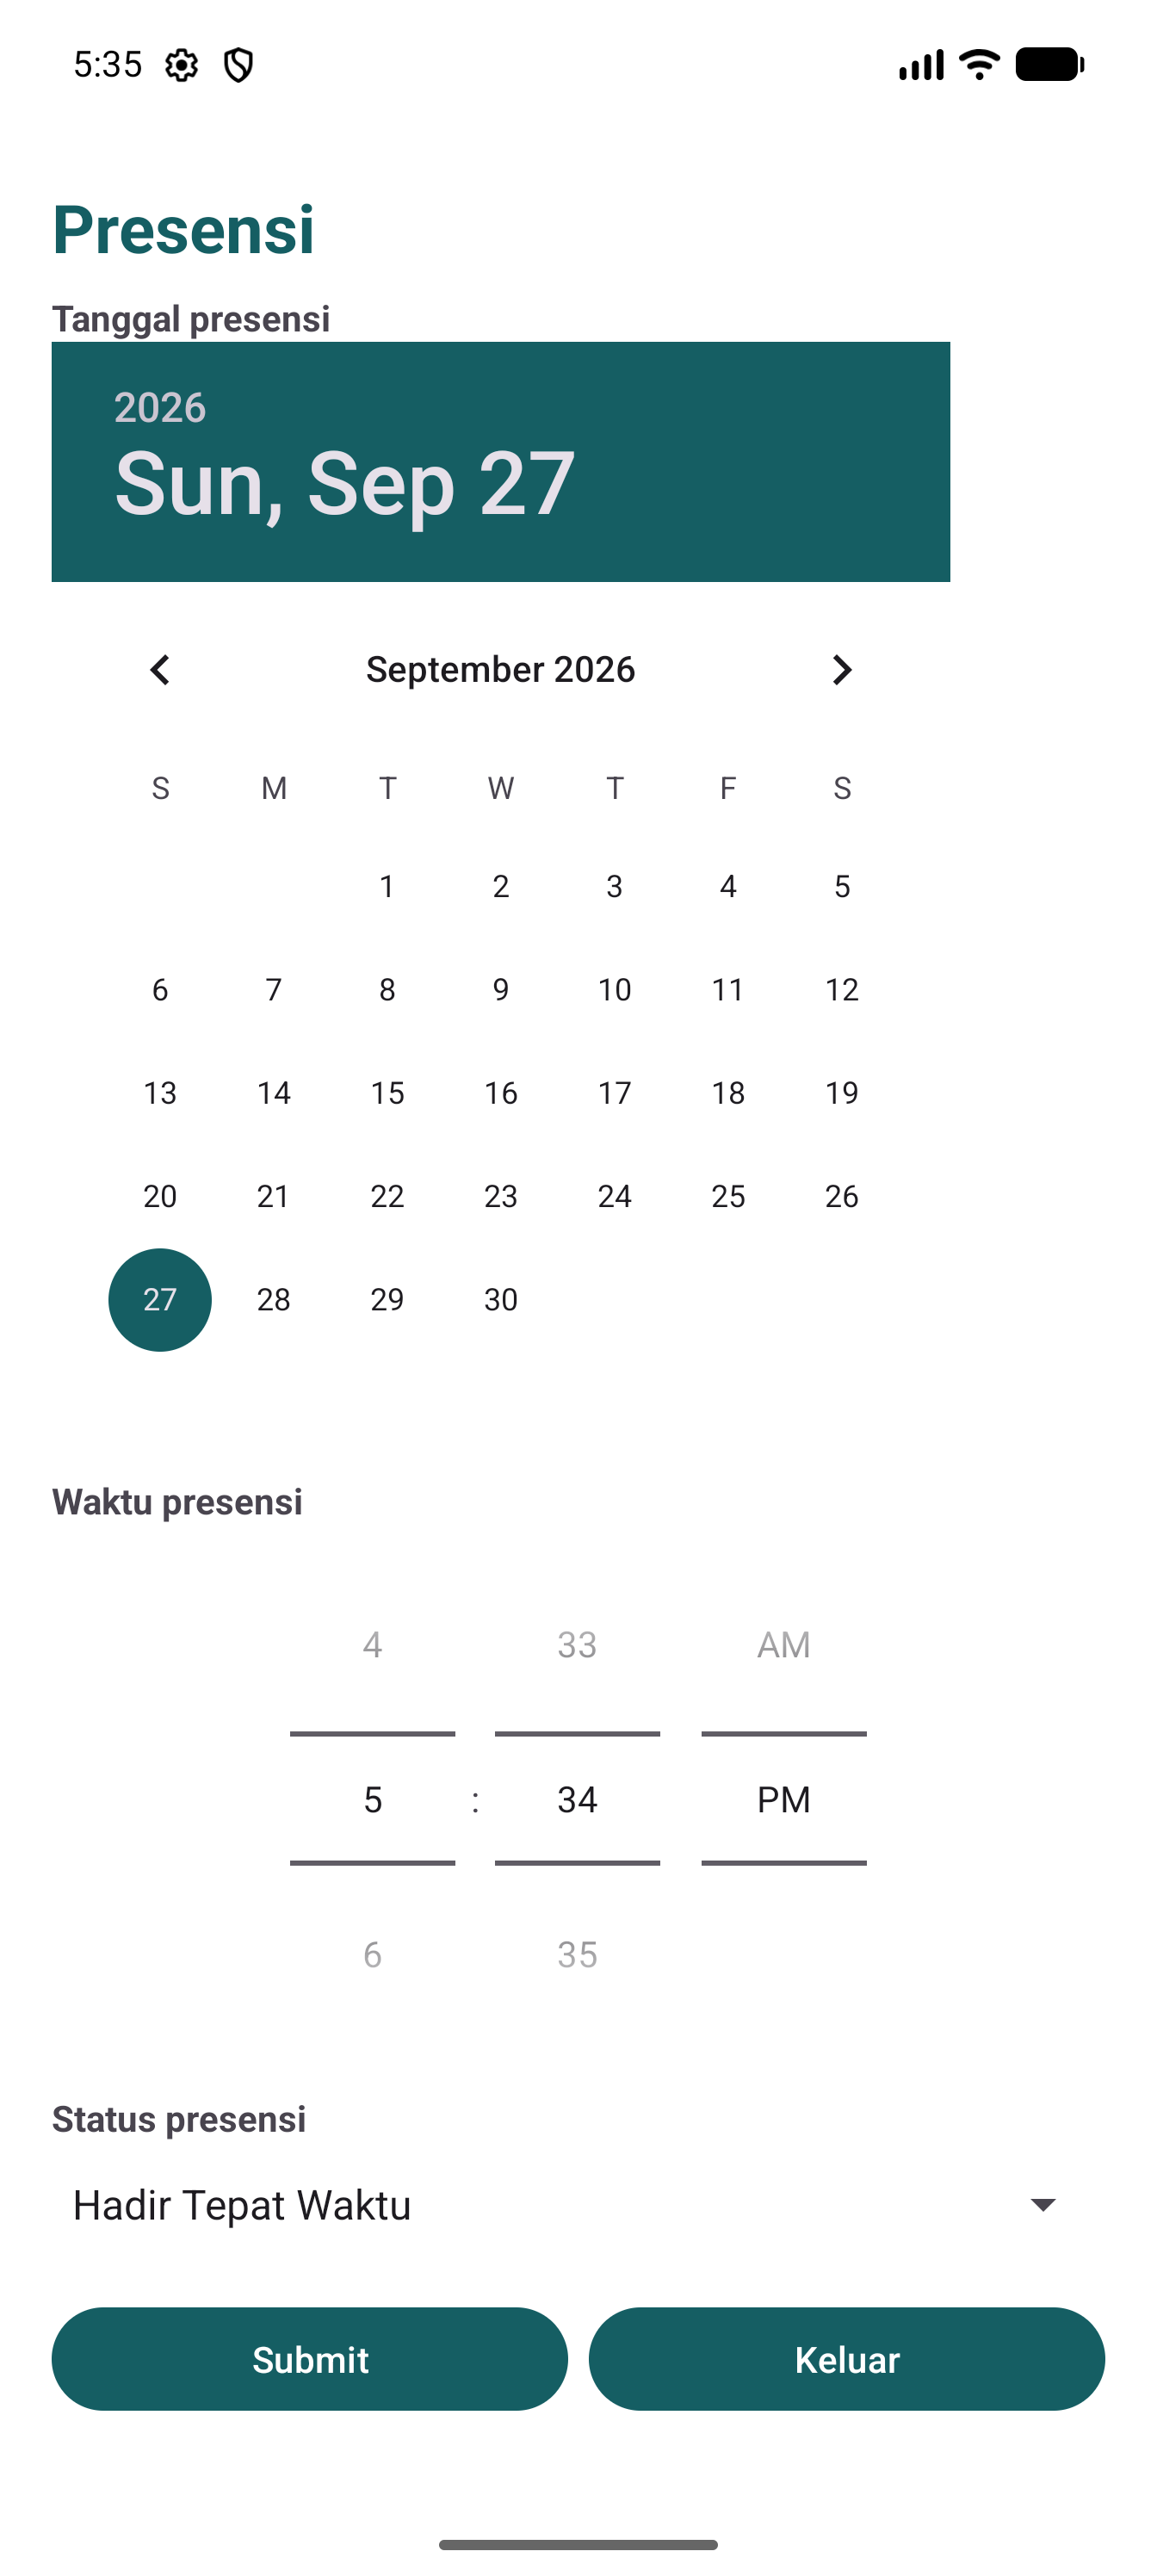
\includegraphics[height=11cm,keepaspectratio]{gambar/01-tampilan-awal.png}\par
\small (a) Tampilan awal aplikasi
\end{minipage}\hfill
\begin{minipage}{0.46\textwidth}\centering
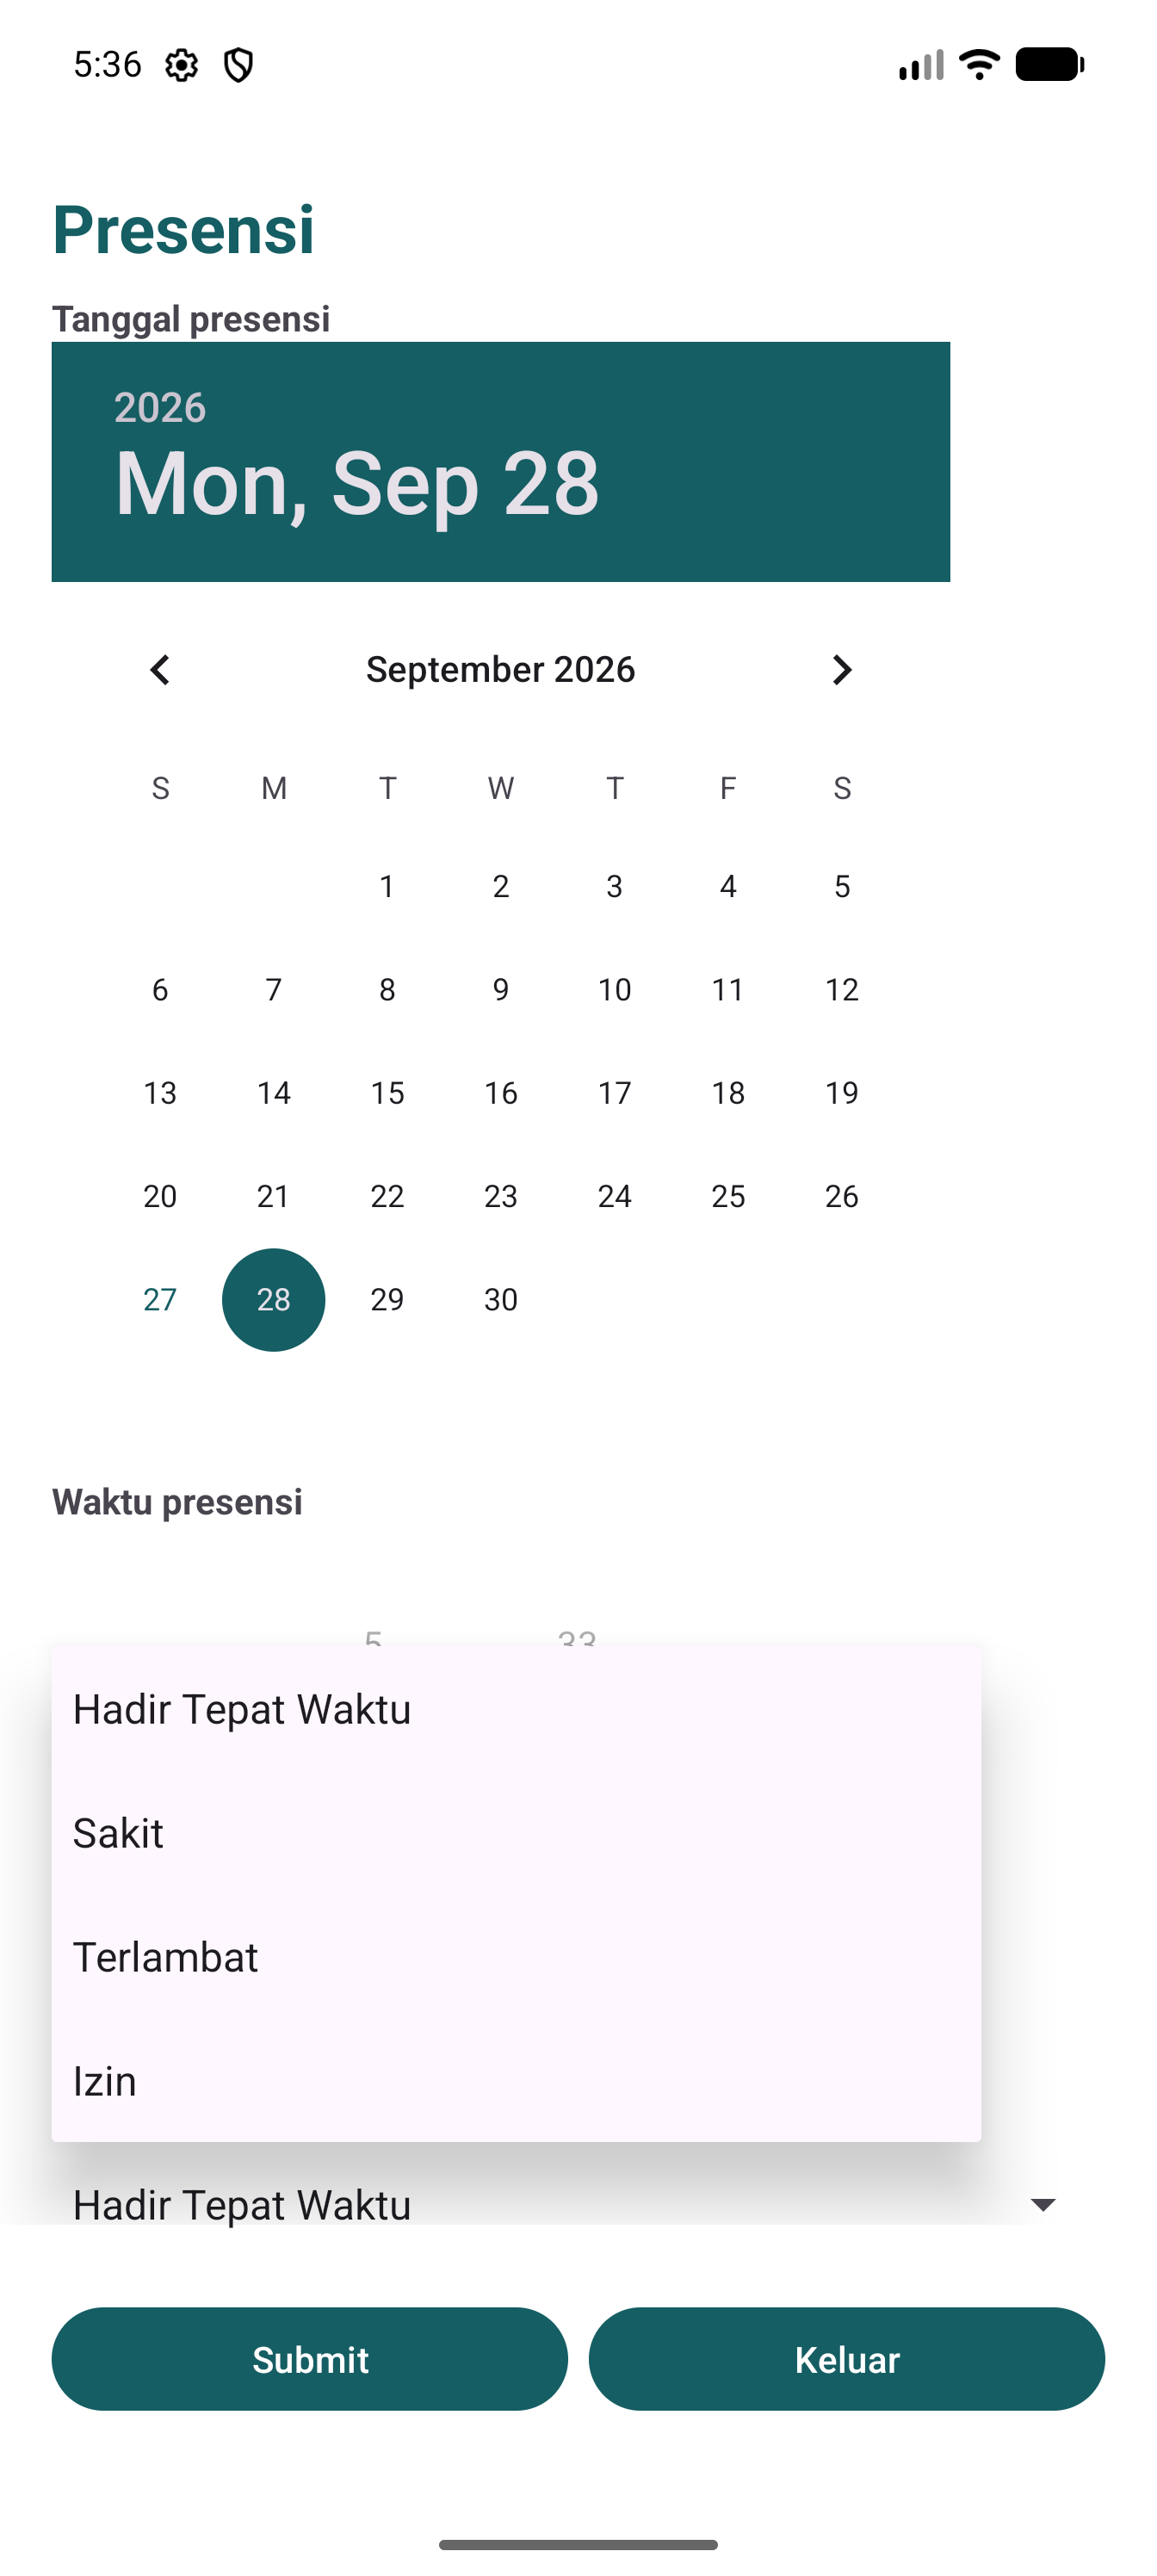
\includegraphics[height=11cm,keepaspectratio]{gambar/02-pilihan-status.png}\par
\small (b) Empat pilihan status
\end{minipage}
\caption{Tampilan awal dan daftar status pada Spinner.}
\end{figure}

\clearpage
\subsection{Kolom Keterangan dan Validasi Input}
Setelah status Sakit dipilih, kolom Keterangan muncul. Pengujian Submit dengan kolom kosong menampilkan pesan ``Isi keterangan terlebih dahulu''. Aplikasi tetap berada pada halaman presensi dan belum menampilkan hasil baru, sehingga input yang belum lengkap dapat diperbaiki.
\begin{figure}[H]
\centering
\begin{minipage}{0.46\textwidth}\centering
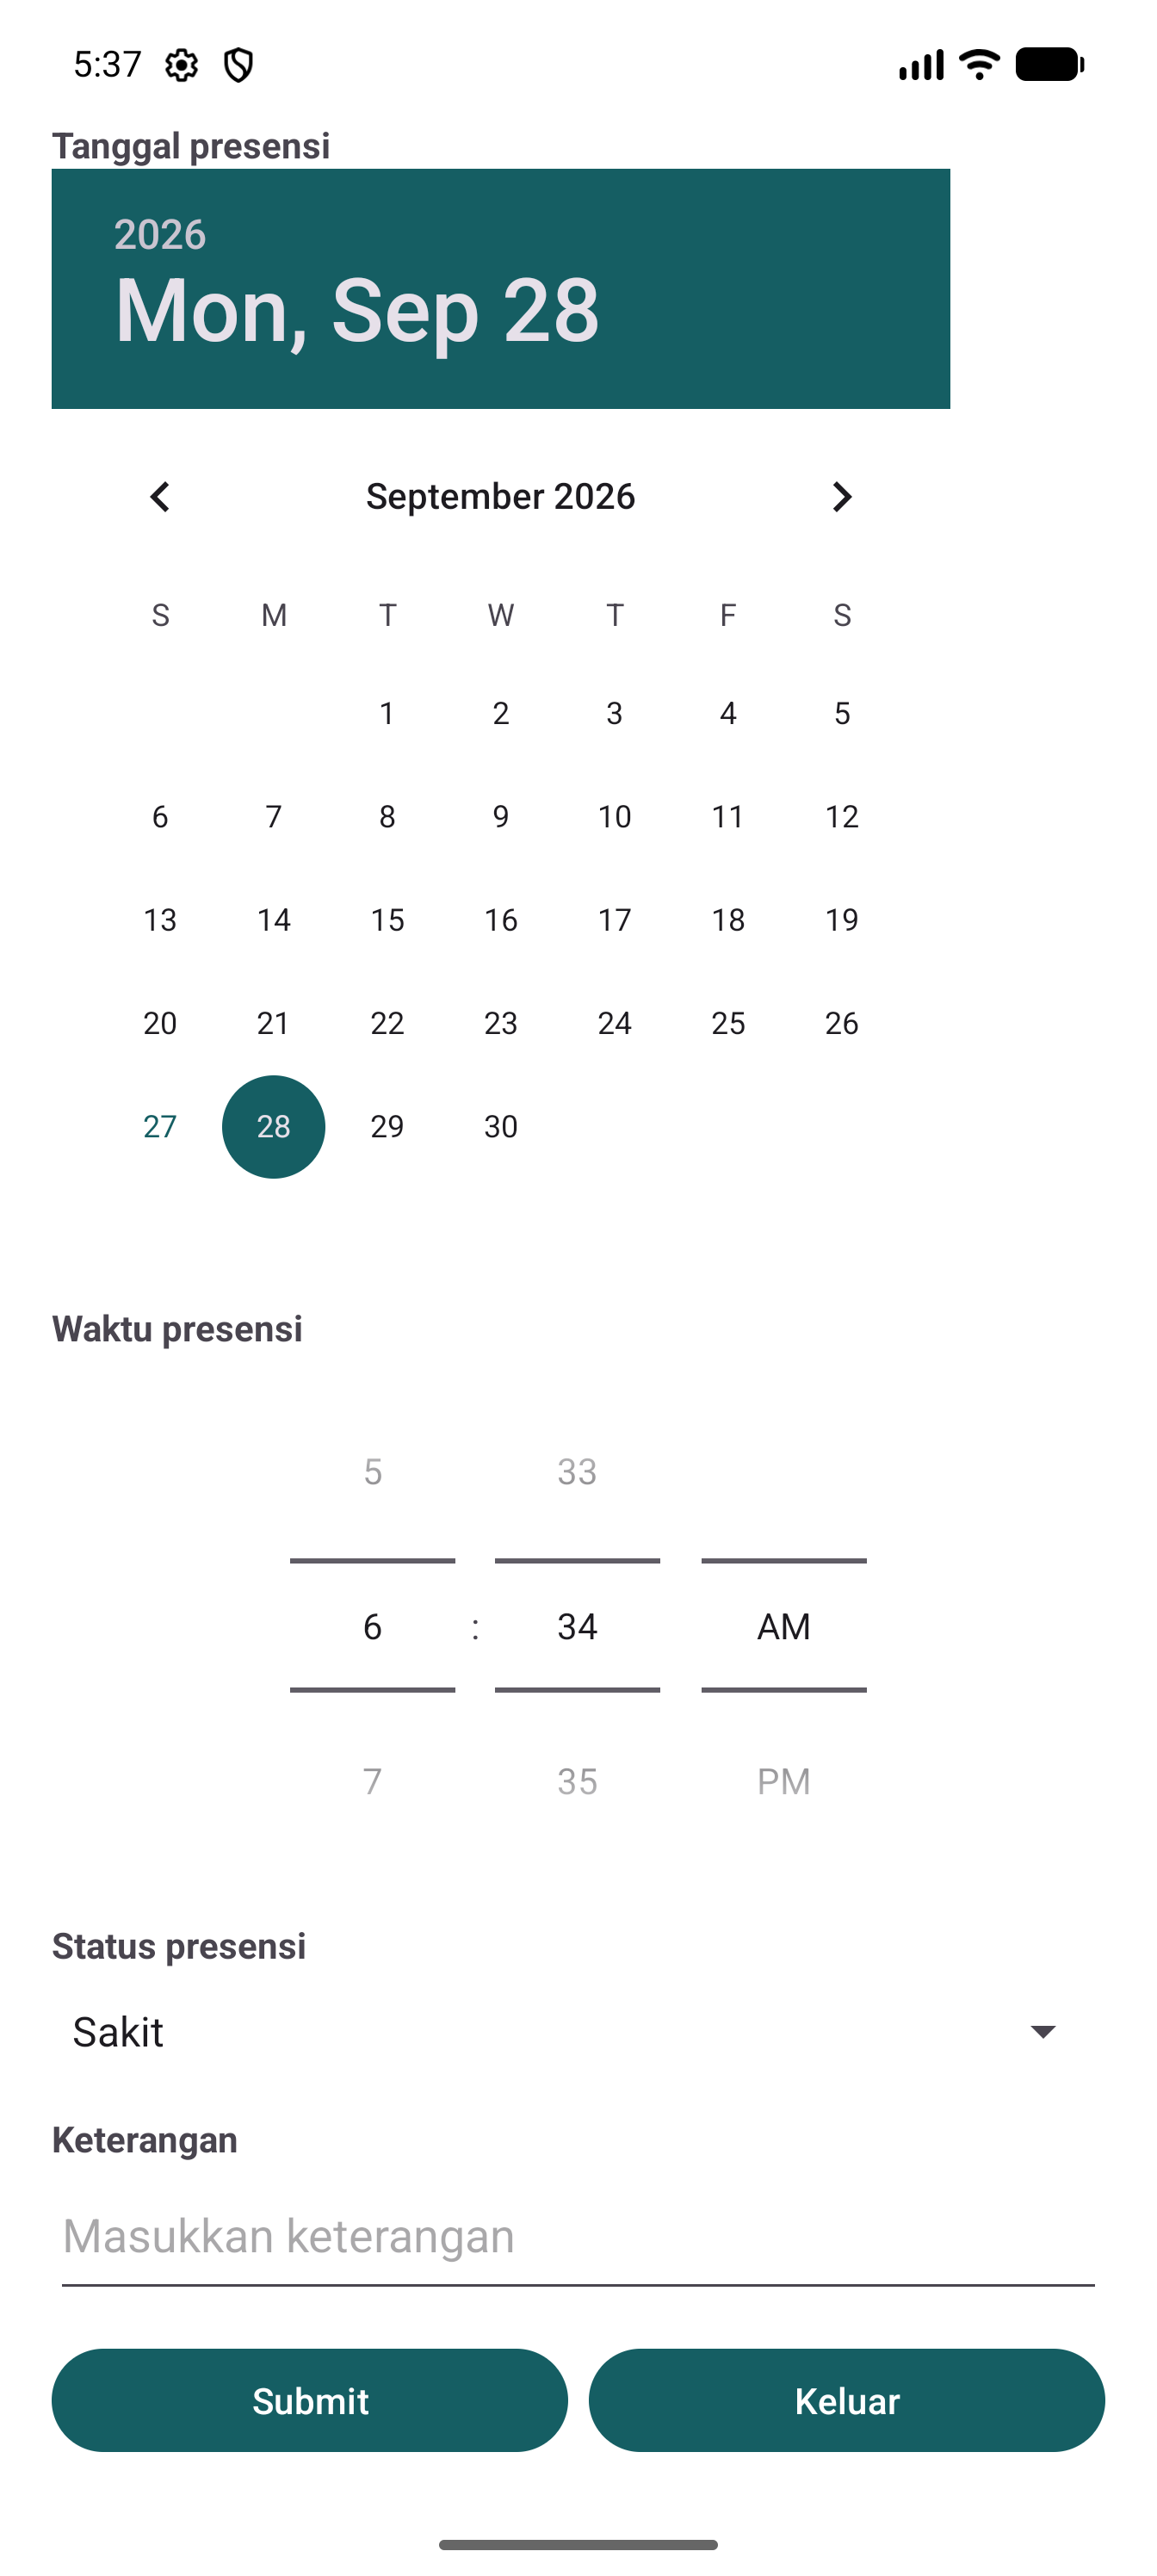
\includegraphics[height=11cm,keepaspectratio]{gambar/03-keterangan-sakit.png}\par
\small (a) Keterangan tampil untuk status Sakit
\end{minipage}\hfill
\begin{minipage}{0.46\textwidth}\centering
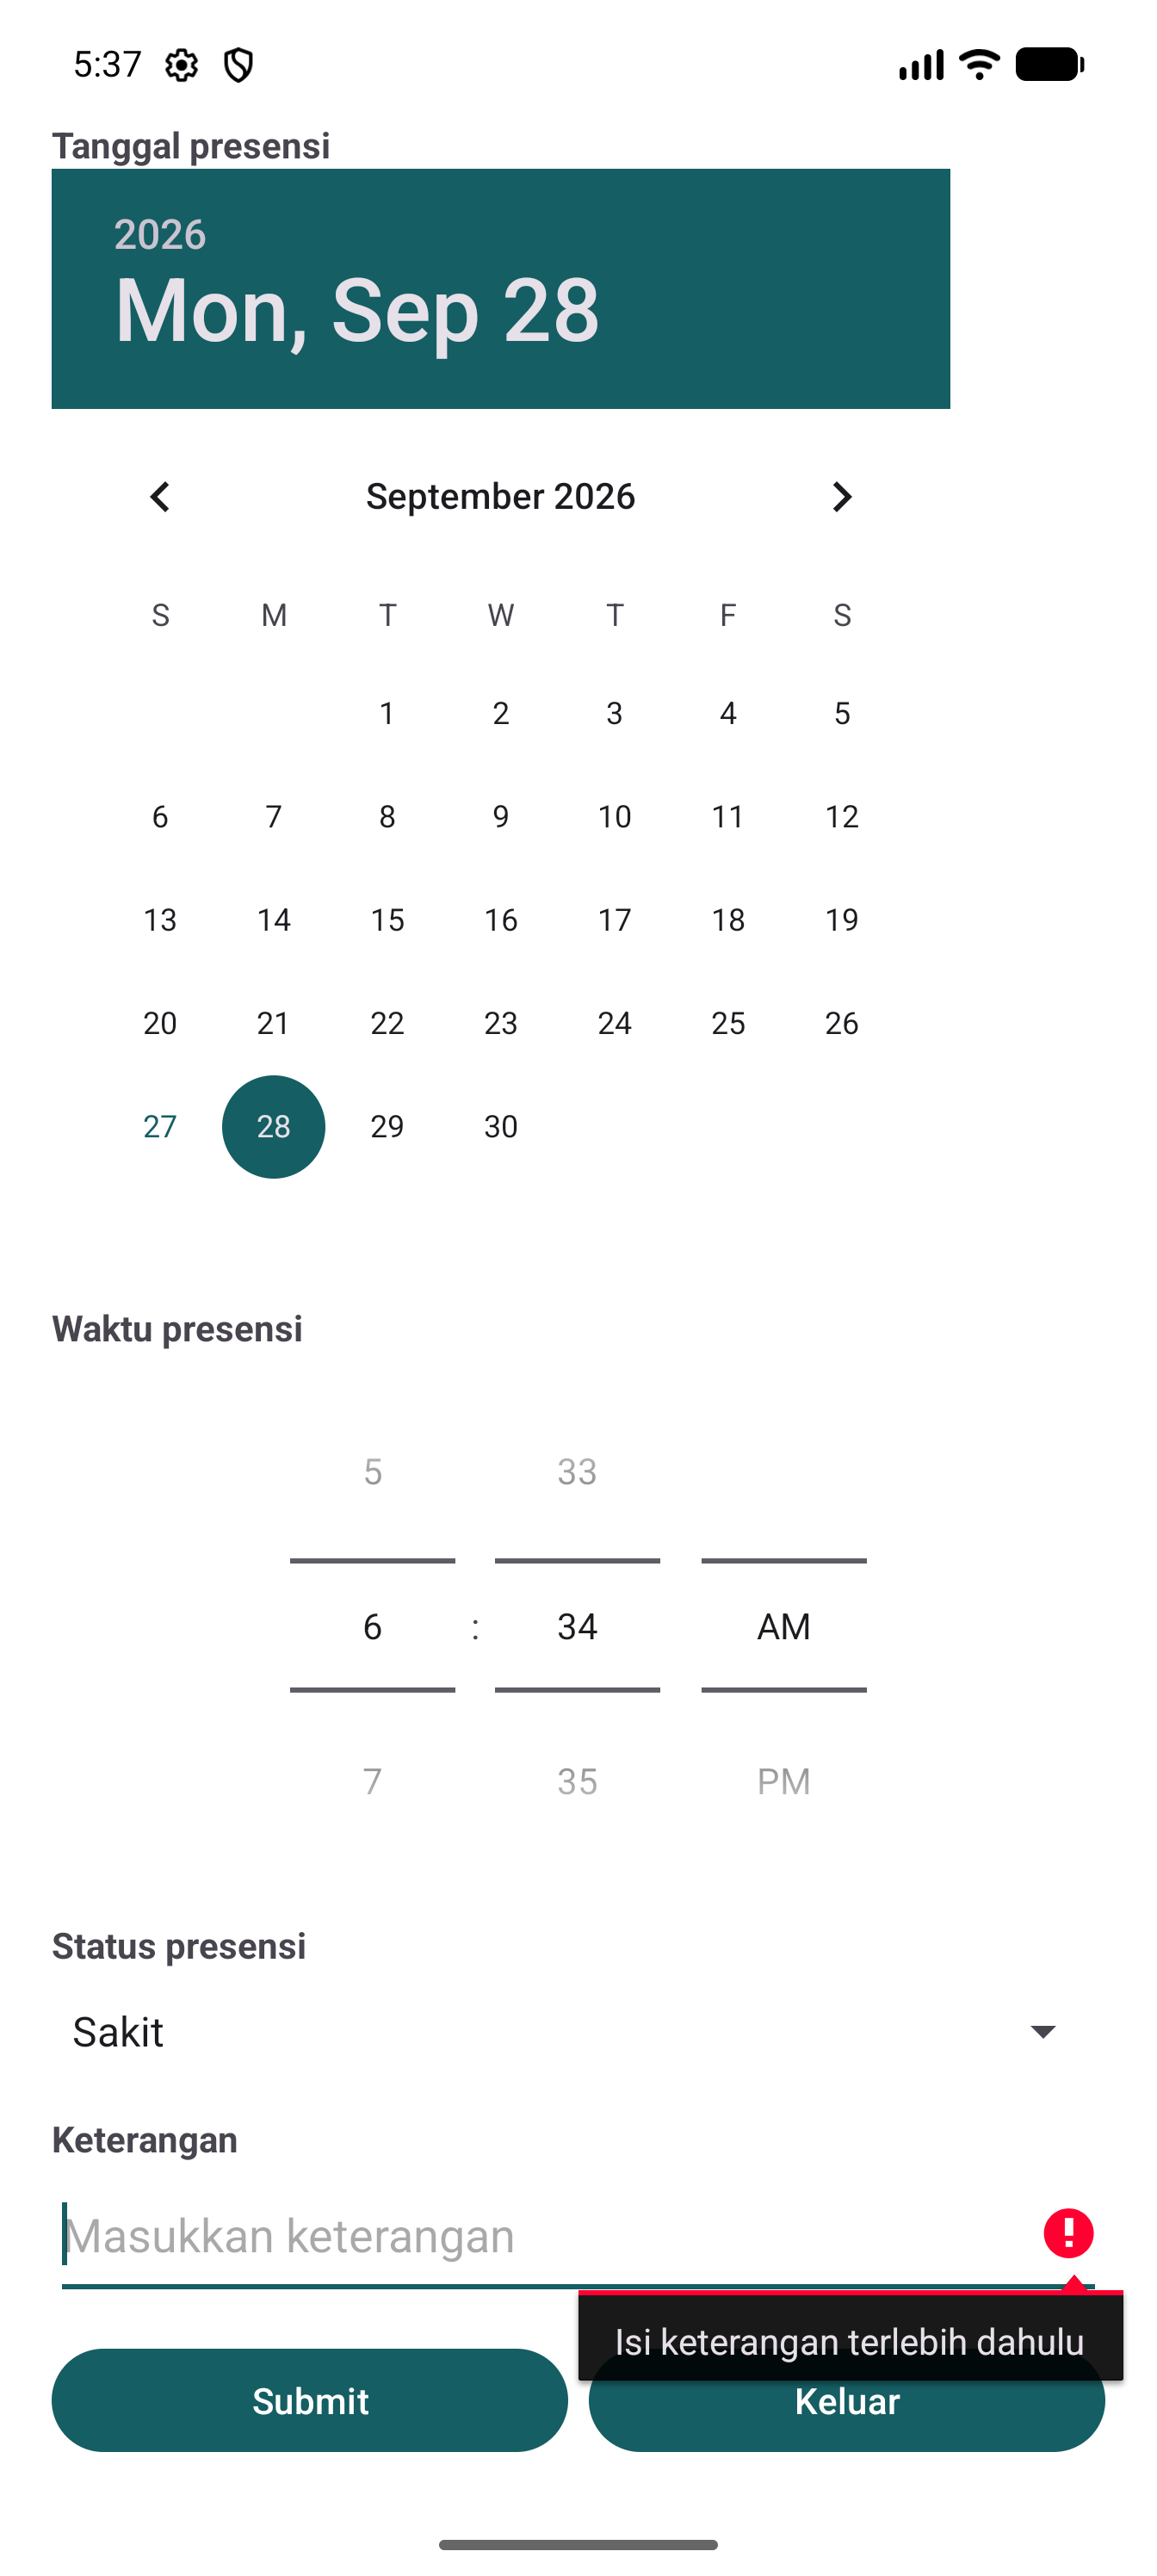
\includegraphics[height=11cm,keepaspectratio]{gambar/04-validasi-keterangan.png}\par
\small (b) Pesan validasi keterangan kosong
\end{minipage}
\caption{Kolom keterangan dinamis dan validasi sebelum Submit.}
\end{figure}

\subsection{Submit Presensi Berhasil}
Pada pengujian status Sakit, keterangan diisi dengan data contoh ``Demam, istirahat sesuai anjuran dokter.''. Setelah Submit, ringkasan menampilkan tanggal 28/09/2026, waktu 06:34 AM, status Sakit, dan keterangan yang dimasukkan. Notifikasi Toast turut muncul. Ketika status diganti menjadi Hadir Tepat Waktu, kolom keterangan disembunyikan dan Submit tetap berhasil tanpa keterangan.

\clearpage
\begin{figure}[H]
\centering
\begin{minipage}{0.46\textwidth}\centering
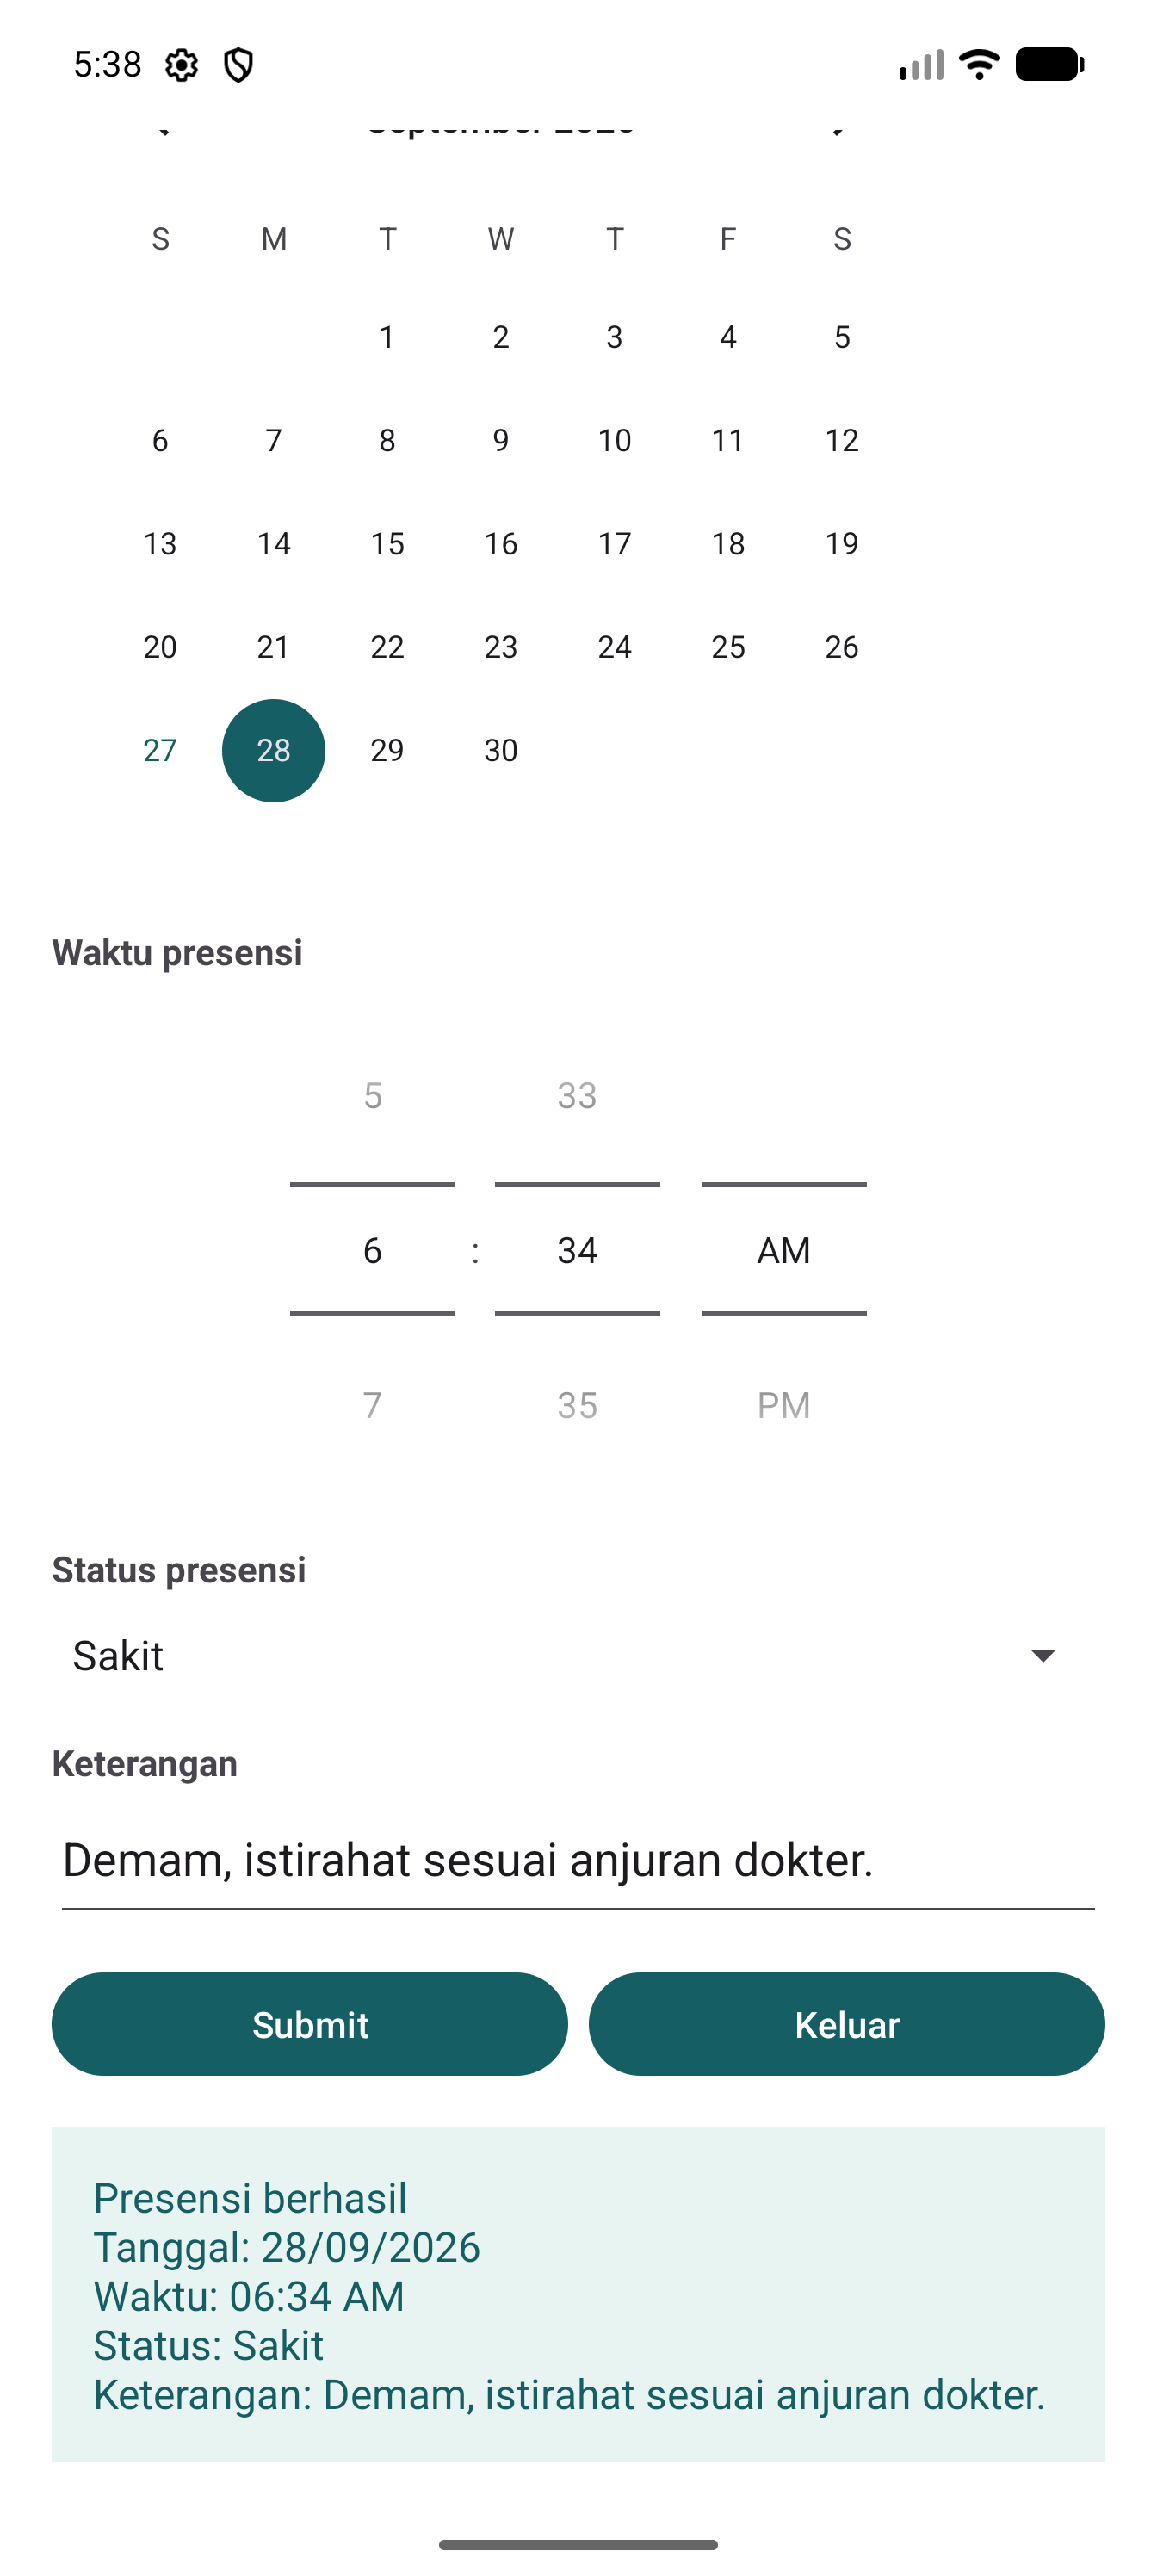
\includegraphics[height=11cm,keepaspectratio]{gambar/05-presensi-berhasil.png}\par
\small (a) Hasil presensi status Sakit
\end{minipage}\hfill
\begin{minipage}{0.46\textwidth}\centering
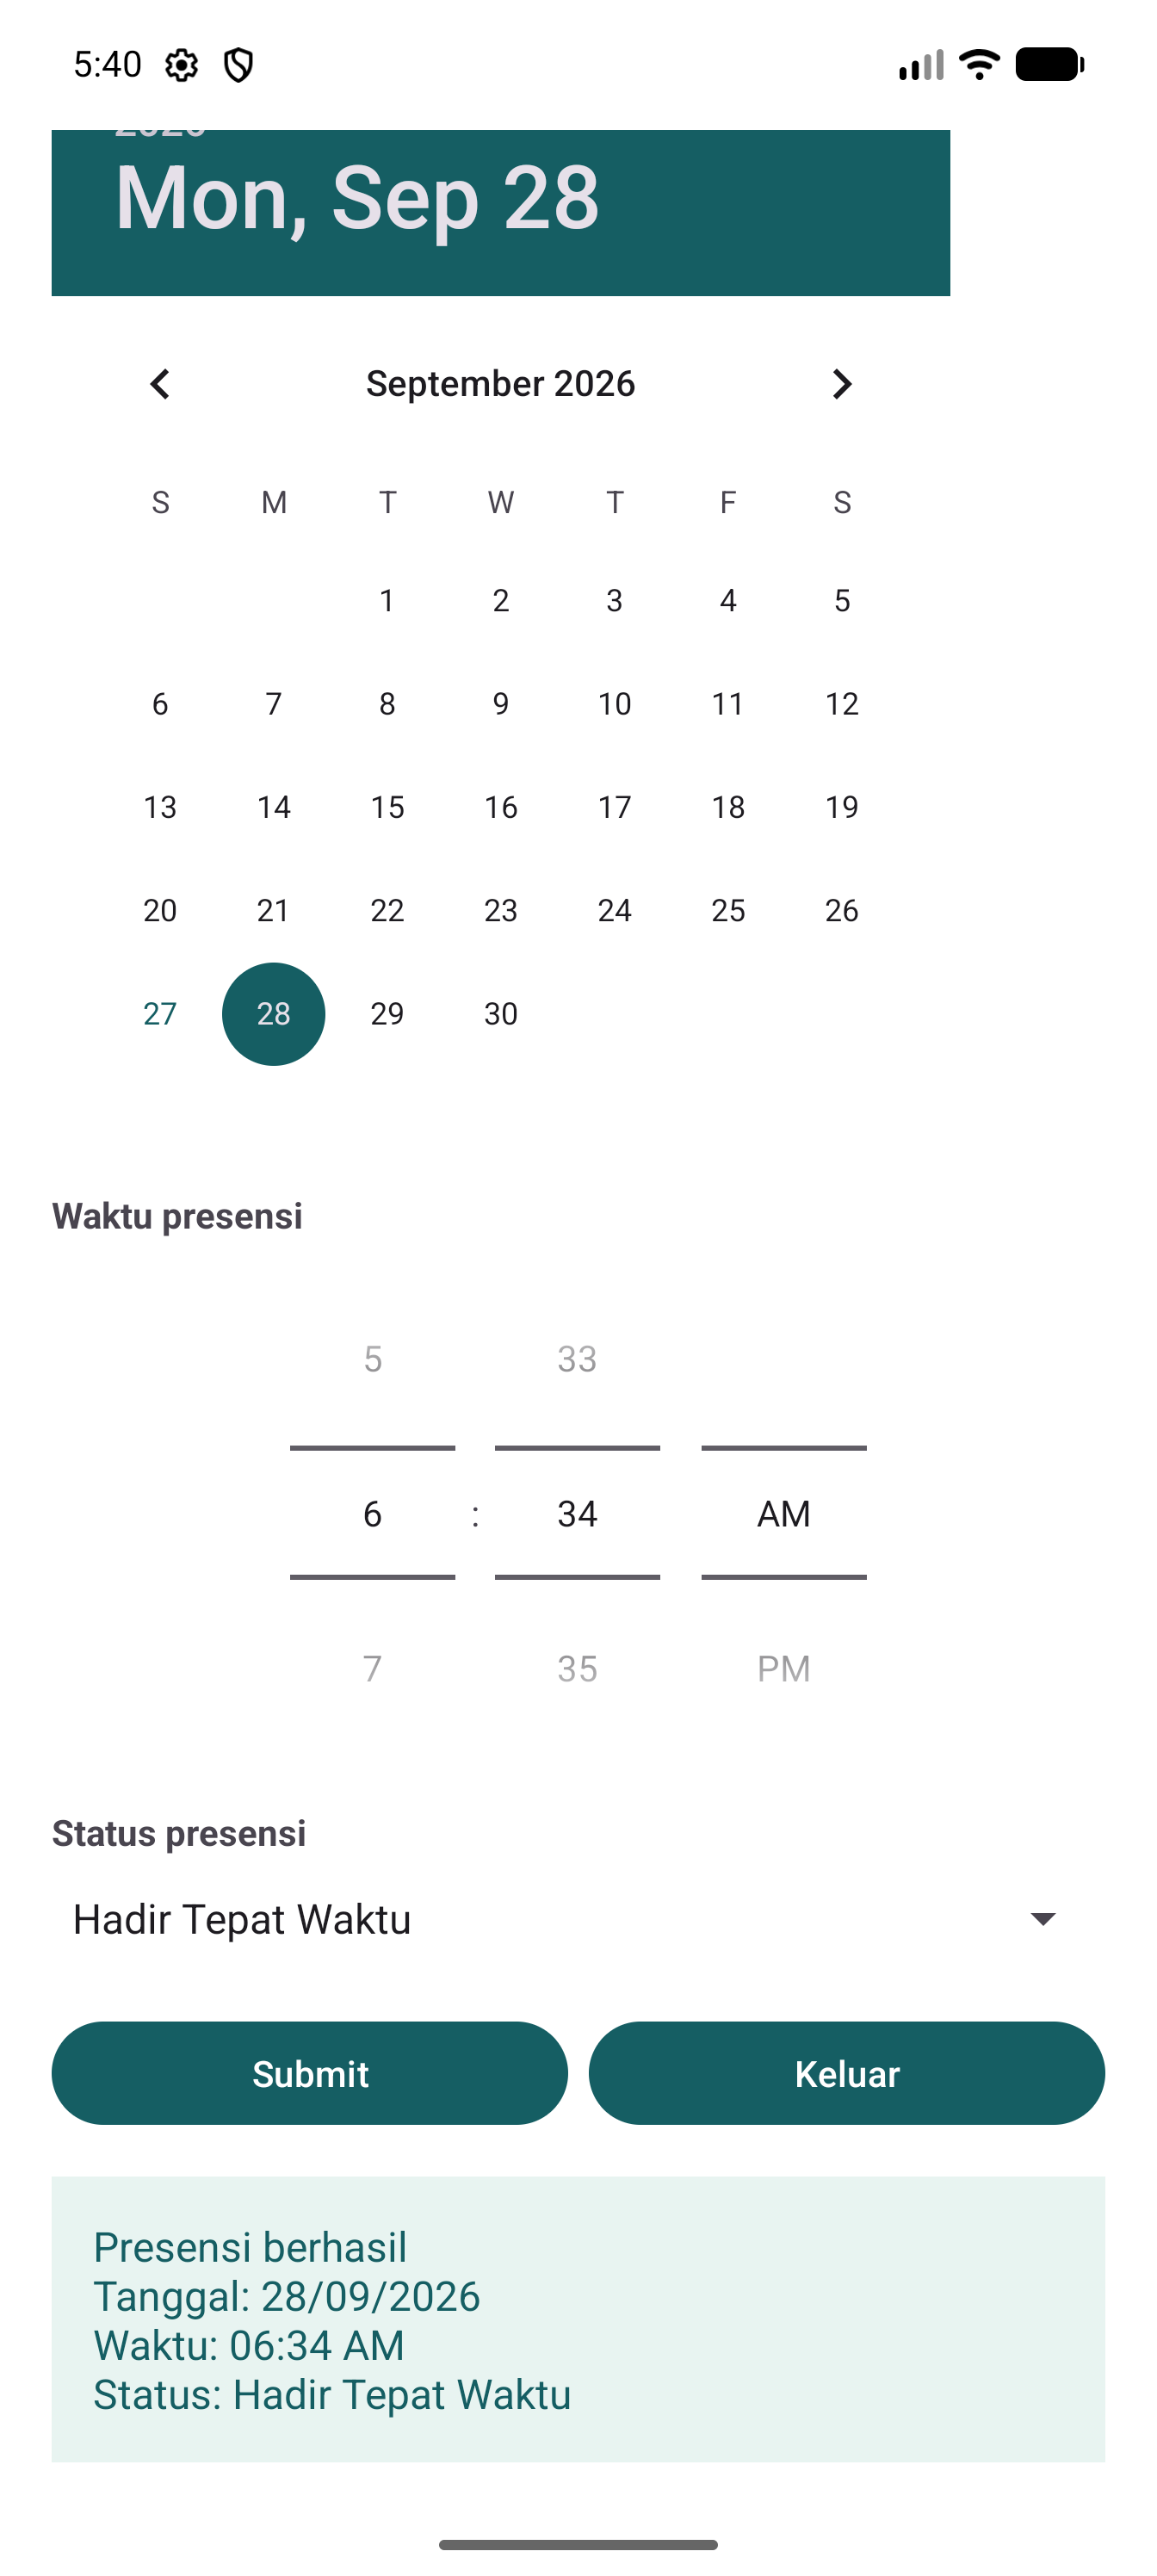
\includegraphics[height=11cm,keepaspectratio]{gambar/07-hadir-tanpa-keterangan.png}\par
\small (b) Hadir berhasil tanpa keterangan
\end{minipage}
\caption{Ringkasan hasil presensi setelah input valid dikirim.}
\end{figure}

\subsection{Konfirmasi Keluar dari Aplikasi}
Saat tombol Keluar ditekan, custom dialog muncul dengan pilihan Tidak dan Ya. Pemilihan Tidak menutup dialog dan mempertahankan halaman presensi. Pemilihan Ya menutup Activity dan mengembalikan emulator ke halaman utama. Alur kedua tombol didokumentasikan pada rekaman demonstrasi.
\begin{figure}[H]
\centering
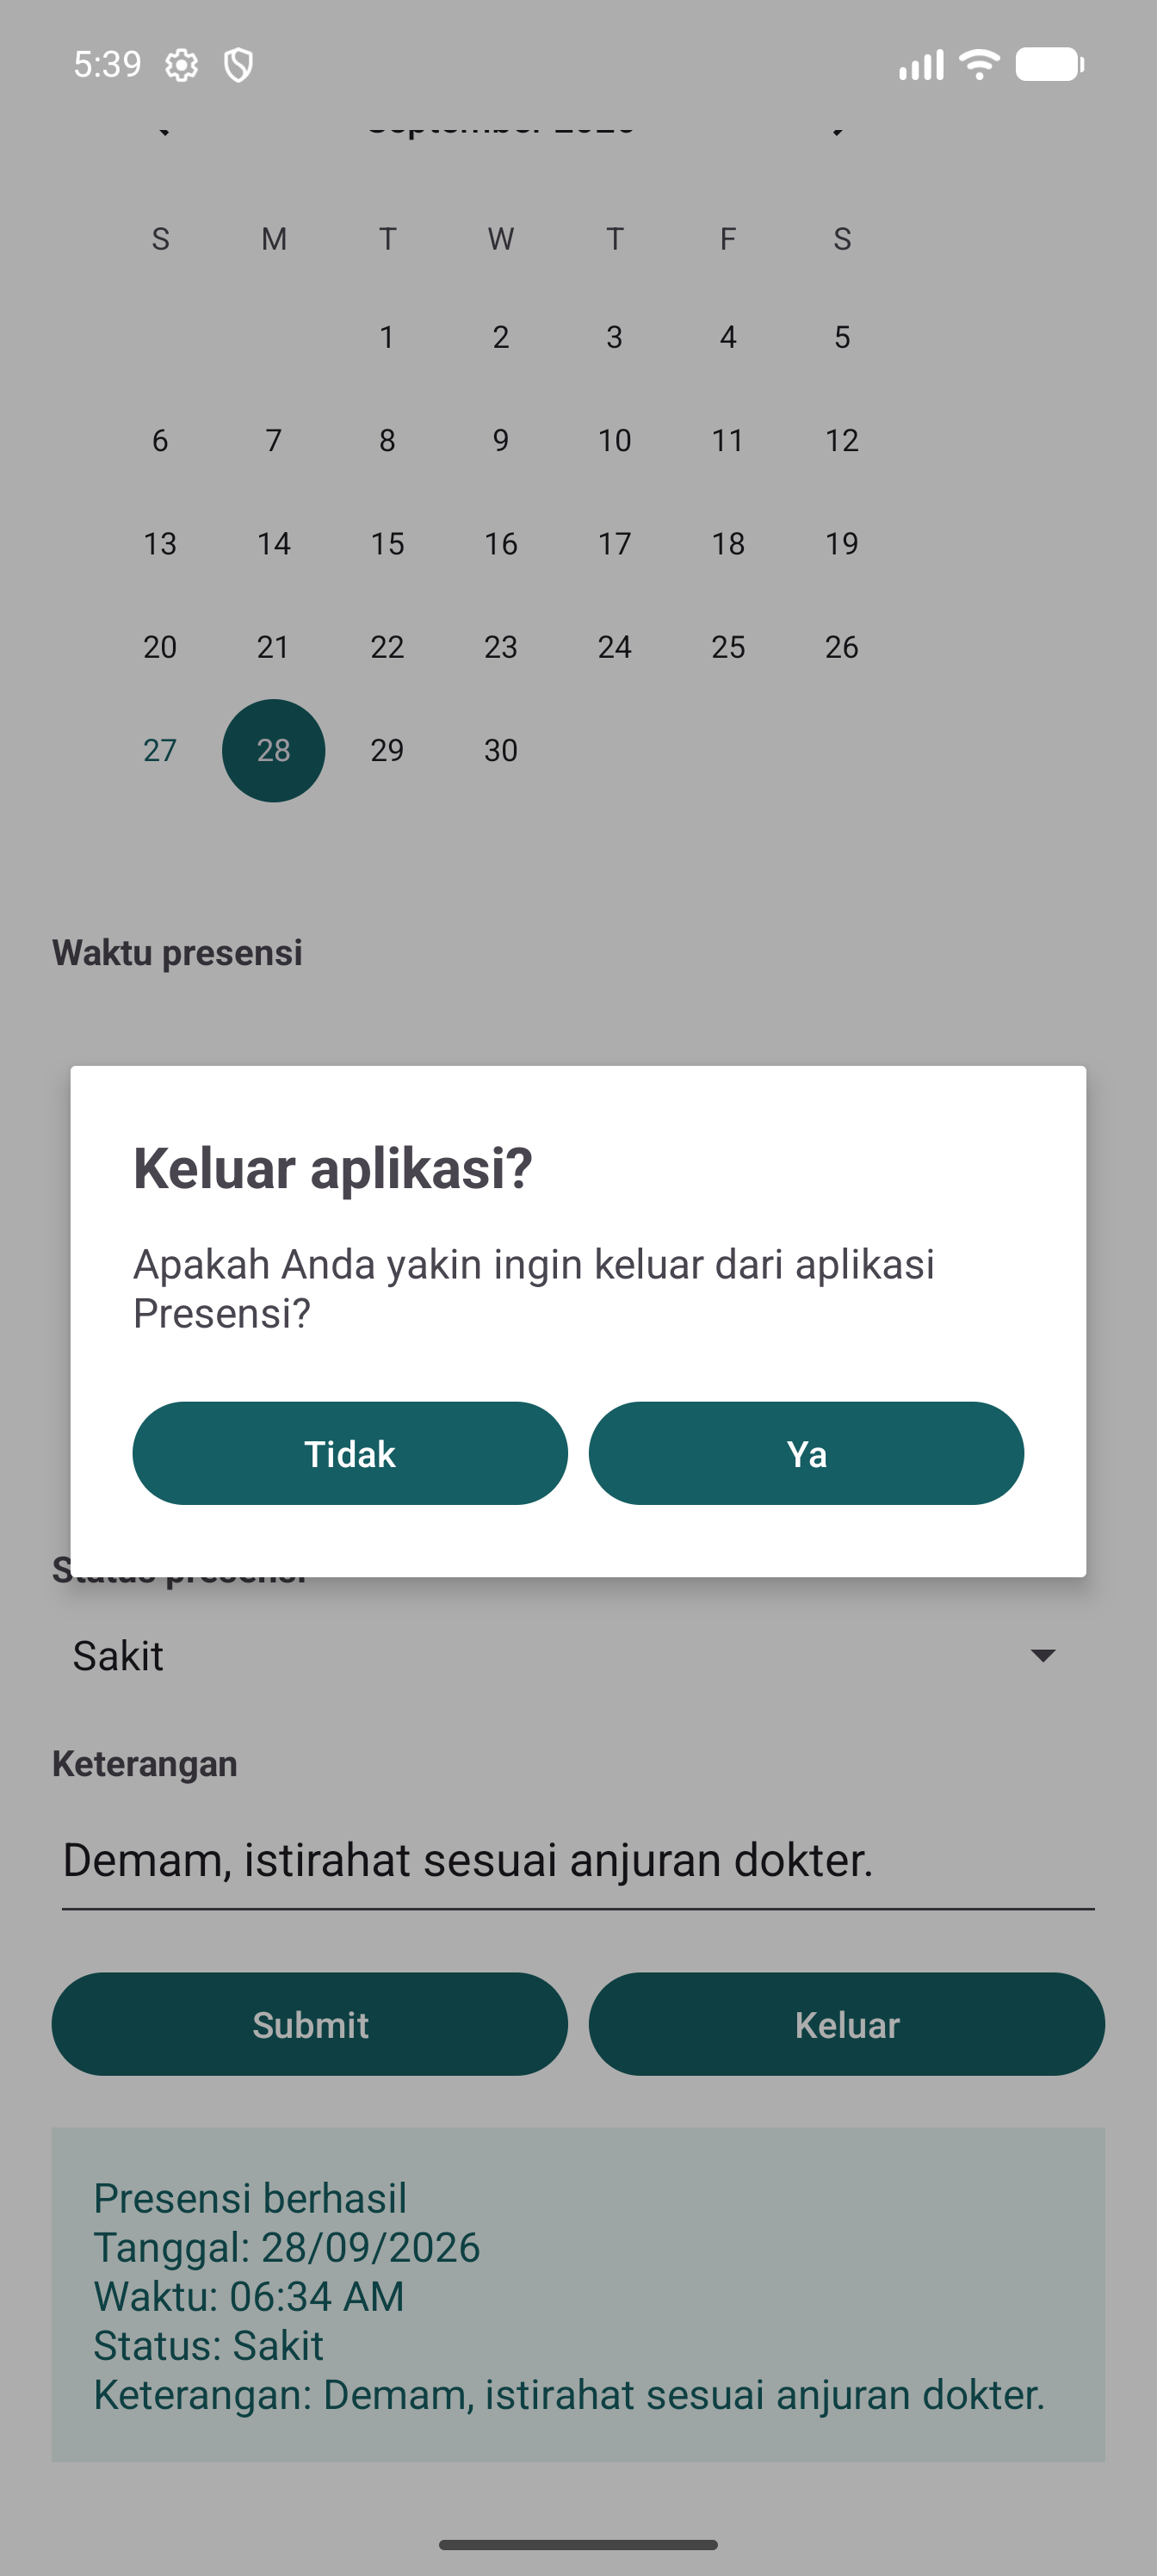
\includegraphics[height=9cm,keepaspectratio]{gambar/06-dialog-keluar.png}
\caption{Custom dialog konfirmasi keluar dari aplikasi.}
\end{figure}

\chapter{Kesimpulan}
Praktikum menghasilkan aplikasi Presensi yang menggabungkan Spinner, DatePicker, TimePicker, View Binding, dan custom dialog. Spinner menyediakan empat status presensi, sedangkan DatePicker dan TimePicker memungkinkan tanggal serta waktu dipilih dan ditampilkan kembali pada hasil Submit.

Kolom keterangan ditampilkan untuk status Sakit, Terlambat, dan Izin, serta disembunyikan untuk Hadir Tepat Waktu. Pengujian status Sakit dengan keterangan kosong memperlihatkan bahwa validasi mencegah input yang belum lengkap dikirim. Pengujian dengan keterangan lengkap dan status Hadir Tepat Waktu menghasilkan ringkasan yang sesuai dengan data pilihan.

Custom dialog memberikan konfirmasi sebelum pengguna keluar. Tombol Tidak mempertahankan aplikasi, sedangkan tombol Ya menutup Activity. Data presensi pada praktikum ini ditampilkan melalui Toast dan TextView; belum disimpan ke database atau dikirim ke server. Dengan demikian, aplikasi memenuhi latihan antarmuka dan penanganan input pada modul.

\chapter{Video}
Rekaman demonstrasi aplikasi tersedia pada file berikut dalam paket hasil praktikum:
\begin{center}
\href{../Video/demo-presensi.mp4}{\textbf{Buka video demonstrasi aplikasi Presensi}}
\end{center}
\noindent\texttt{Video/demo-presensi.mp4}

Video merupakan rekaman layar emulator tanpa narasi suara. Demonstrasi memperlihatkan pemilihan tanggal dan waktu, daftar status, kemunculan kolom keterangan, validasi input kosong, hasil Submit, dan custom dialog keluar. Rekaman asli juga disertakan di folder Video untuk meninjau urutan pengujian secara lengkap. File MP4 dapat diunggah ke layanan video sesuai ketentuan pengumpulan praktikum apabila diperlukan tautan daring.
\end{document}
